\documentclass[11pt,journal]{IEEEtran}
\usepackage{amsmath}
\usepackage{graphicx}
\usepackage{listings}

\graphicspath{{./}}

\title{Emotion Recogniser}

\author{Tianqi (Carl) Liu, ~\IEEEmembership{z5019791} \\
        Han Zhang Zeng, ~\IEEEmembership{z12345678}}

\begin{document}
\maketitle
\begin{abstract}
    This is a report on the emotion recognizer project for comp9517 at UNSW. the report includes our goal, reference survey, problem decomposition, detailed specification, design, test and group contribution and conclusion.
\end{abstract}
\section{Introduction}
  The goal of the project is to able to recognize human emotion on real time live stream to a degree of accuracy (at the start of the project we set the benchmark to around 50\%). There are 4 emotions that we are concerned with:
  \begin{enumerate}
    \item neutral
    \item happy
    \item angry
    \item sadness
  \end{enumerate}
  other: when the recognizer is not sure we consider the emotion to be some other emotion\\\\
  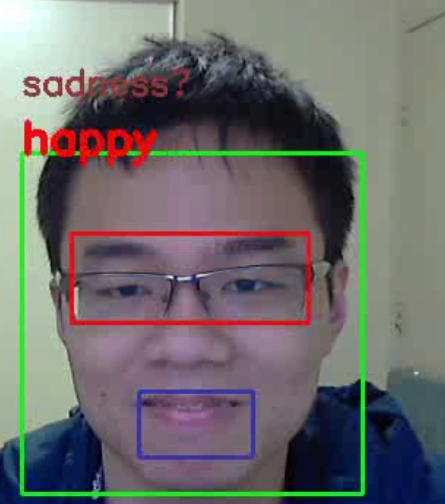
\includegraphics[width=0.4\textwidth]{01.png} \\\\
  As shown in the photo, there are 2 emotions displayed. The larger text on top of the frame is the best estimation of the current emotion, the dark red text is the 2nd best predication.

\section{Problem Decomposition}
  The project consists of two major components:
  \begin{enumerate}
    \item Face Extraction
    \item Emotion Recognition
  \end{enumerate}

  \subsection{Face Extraction}
    In order to perform the emotion recoginition algorithm, we need to extract the face from the image
\end{document}
